% -*- TeX-engine: luatex -*-

% Your presentation should consist of an overview of your research
% achievements, plans and vision, outlining how your work would
% contribute to the University and who you could collaborate with at
% Strathclyde.

% High performance numerical software;
% structure-preserving discretisation;
% preconditioning
% Plans: high order methods: automation, hp-adaptivity
% Strathclyde collaboration:
% - Barranchea (discretisation -> preconditioning)
% - Dolean (preconditioning [DD not multigrid...])
% - Majumdar (liquid crystals, FEM)

% Background: finite element methods, automation (assembly)
% Preconditioning: optimal algorithms, composable implementation
% Significance: first general implementation of many state-of-the-art
% multigrid smoothers

\documentclass[presentation,aspectratio=43, 10pt]{beamer}
\usepackage{pifont}
\newcommand{\cmark}{\ding{51}}
\newcommand{\xmark}{\ding{55}}
\usepackage{standalone}
\usepackage{booktabs}
% \titlegraphic{\hfill
\includegraphics[height=1.25cm]{durham-logo}}
\usepackage{appendixnumberbeamer}
\def\xunderbrace#1_#2{{\underbrace{#1}_{\mathclap{#2}}}}
\def\xoverbrace#1^#2{{\overbrace{#1}^{\mathclap{#2}}}}
\def\xunderarrow#1_#2{{\underset{\overset{\uparrow}{\mathclap{#2}}}{#1}}}
\def\xoverarrow#1^#2{{\overset{\underset{\downarrow}{\mathclap{#2}}}{#1}}}
\usepackage{amsmath}
\usepackage{amssymb}
\usepackage{mathtools}
\usepackage{hyperref}
\usepackage{xspace}
\newcommand{\arxivlink}[2]{{\texttt{arXiv:\,\href{https://arxiv.org/abs/#1}{#1\,[#2]}}}}

\newcommand{\honev}{\ensuremath{{H}^1(\Omega; \mathbb{R}^d)}\xspace}
\newcommand{\ltwov}{\ensuremath{{L}^2(\Omega; \mathbb{R}^d)}\xspace}
\newcommand{\ltwo}{\ensuremath{{L}^2(\Omega)}\xspace}
\newcommand{\inner}[1]{\left\langle #1 \right \rangle}
\newcommand{\advect}[2]{\ensuremath{(#2 \cdot \nabla) #1}}
\newcommand{\kerdiv}{\ker\div}
\newcommand{\eps}[1]{\ensuremath{\varepsilon{(#1)}}}
\newcommand{\kercurl}{\ker\curl}
\newcommand{\dx}{\ \text{d}x}
\newcommand{\ds}{\ \text{d}s}
\newcommand{\Pq}{\ensuremath{\mathrm{P}_{Q_h}}}
\newcommand{\PqK}{\ensuremath{\mathrm{P}_{Q_h(K)}}}
\newcommand{\Ptwo}{\ensuremath{\mathbb{P}_2}\xspace}
\newcommand{\Pthree}{\ensuremath{\mathbb{P}_3}\xspace}
\newcommand{\PtwoPzero}{\ensuremath{[\mathbb{P}_2]^2\mathrm{-}\mathbb{P}_0}\xspace}
\newcommand{\PtwothreePzero}{\ensuremath{[\mathbb{P}_2]^3\mathrm{-}\mathbb{P}_0}\xspace}
\newcommand{\PthreePzero}{\ensuremath{[\mathbb{P}_3]^3\mathrm{-}\mathbb{P}_0}\xspace}
\newcommand{\Pzero}{\ensuremath{\mathbb{P}_0}\xspace}
\newcommand{\Pv}{\ensuremath{\mathbb{P}_v}\xspace}
\newcommand{\BR}{\ensuremath{\left[\mathbb{P}_1 \oplus B^F_3\right]}\xspace}
\newcommand{\PoneFB}{\ensuremath{\mathbb{P}_1 \oplus B^F_3}\xspace}
\newcommand{\PtwoFB}{\ensuremath{\mathbb{P}_2 \oplus B^F_3}\xspace}
\newcommand{\BRzero}{\ensuremath{\BR^3\mathrm{-}\mathbb{P}_0}\xspace}
\newcommand{\fmw}{\ensuremath{\left(\mathbb{P}_2 \oplus B^F_3\right)}\xspace}
\newcommand{\fmwzero}{\ensuremath{\fmw^3\mathrm{-}\mathbb{P}_0}\xspace}
\setbeamersize{text margin left=0.5cm, text margin right=0.5cm}
\let\Re\relax
\DeclareMathOperator{\Re}{Re}


\usepackage{minted}
\usepackage[url=false,
doi=true,
isbn=false,
style=authoryear,
maxnames=5,
giveninits=true,
uniquename=init,
backend=biber]{biblatex}
\renewcommand{\bibfont}{\fontsize{7}{7}\selectfont}
\addbibresource{../literature.bib}
\setbeamertemplate{bibliography item}[triangle]
\defbibenvironment{bibliography}
  {\list{}
     {\settowidth{\labelwidth}{\usebeamertemplate{bibliography item}}%
      \setlength{\leftmargin}{\labelwidth}%
      \setlength{\rightmargin}{\labelwidth}%
      \setlength{\labelsep}{\biblabelsep}%
      \addtolength{\leftmargin}{\labelsep}%
      \setlength{\itemsep}{\bibitemsep}%
      \setlength{\parsep}{\bibparsep}}}
  {\endlist}
  {\item}
\setlength{\bibitemsep}{1ex}
\setlength{\fboxsep}{1pt}

\renewbibmacro{in:}{}
\DeclareFieldFormat[article]{volume}{\textbf{#1}}
\DeclareFieldFormat{doi}{%
  doi\addcolon%
  {\scriptsize\ifhyperref{\href{http://dx.doi.org/#1}{\nolinkurl{#1}}}
    {\nolinkurl{#1}}}}
\AtEveryBibitem{%
\clearfield{pages}%
\clearfield{issue}%
\clearfield{number}%
}

\newcommand{\grad}{\ensuremath{\nabla}}
\let\div\relax
\DeclareMathOperator{\div}{div}
\DeclareMathOperator{\curl}{curl}
\DeclareMathOperator{\range}{range}
\DeclareMathOperator{\sym}{sym}
\usetheme{metropolis}
\setbeamertemplate{title graphic}{
  \vbox to 0pt {
    \vspace*{1em}
    \inserttitlegraphic%
  }%
  \nointerlineskip%
}
\metroset{background=light,progressbar=frametitle,numbering=counter,block=fill}

% https://www.dur.ac.uk/marketingandcommunications/marketing/branding/colourpalette/
% Most of these are indistinguishable to those suffering colour blindness
\definecolor{purple}{HTML}{68246D}
\definecolor{blue}{HTML}{002A41}
\definecolor{red}{HTML}{BE1E2D}
\definecolor{cyan}{HTML}{00AEEF}
\definecolor{yellow}{HTML}{00AA1A}

\newenvironment{variableblock}[3]
{\setbeamercolor{block body}{#2}
\setbeamercolor{block title}{#3}
\begin{block}{#1}}%
{\end{block}}
  
\newenvironment{challenge}[1]%
{\begin{variableblock}{#1}{bg=red!20,fg=black}{bg=red,fg=white}}%
{\end{variableblock}}

\newenvironment{answer}[1]%
{\begin{variableblock}{#1}{bg=cyan!20,fg=black}{bg=cyan,fg=white}}%
{\end{variableblock}}

\renewenvironment{exampleblock}[1]%
{\begin{variableblock}{#1}{bg=yellow!20,fg=black}{bg=yellow,fg=white}}%
{\end{variableblock}}

\setbeamercolor{normal text}{
  fg=black,
  bg=white
}
\setbeamercolor{alerted text}{
  fg=red
}
\setbeamercolor{example text}{
  fg=blue
}

\setbeamercolor{palette primary}{%
  use=normal text,
  fg=normal text.bg,
  bg=purple,
}

\usetheme{metropolis}

\author{Lawrence Mitchell\inst{1,*}}
\institute{
  \inst{1}Department of Computer Science, Durham University\\
  \inst{*}\texttt{lawrence.mitchell@durham.ac.uk}}

\date{26th April 2021}
\title{Symbolics and structure: fast finite elements and preconditioning}

\usepackage{tikz}
\usetikzlibrary{trees,calc,positioning}
\usetikzlibrary{shapes, shapes.geometric}
\usetikzlibrary{arrows,chains,positioning,fit,backgrounds,calc,shapes,
  shadows,scopes,decorations.markings,plotmarks}
\usepackage{tikz-cd}
\usepackage{pgf}
\usepackage{pgfplots}
\usepackage{pgfplotstable}

\newcommand*{\tettextsize}{\footnotesize}
\tikzstyle{line} = [draw, -, thick]
\tikzstyle{nodraw} = [draw, fill, circle, minimum width=0pt, inner sep=0pt]
\tikzstyle{sieve} = [line, circle, font=\tettextsize, inner sep=0pt,
  minimum size=12pt]

\tikzstyle{cell} = [sieve, fill=blue!60]
\tikzstyle{facet} = [sieve, fill=green!35]
\tikzstyle{edge} = [sieve, fill=red!35]
\tikzstyle{vertex} = [sieve, fill=blue!35]

% https://tex.stackexchange.com/questions/27171/padded-boundary-of-convex-hull
\newcommand{\convexpath}[2]{
  [
  create hullcoords/.code={
    \global\edef\namelist{#1}
    \foreach [count=\counter] \nodename in \namelist {
      \global\edef\numberofnodes{\counter}
      \coordinate (hullcoord\counter) at (\nodename);
    }
    \coordinate (hullcoord0) at (hullcoord\numberofnodes);
    \pgfmathtruncatemacro\lastnumber{\numberofnodes+1}
    \coordinate (hullcoord\lastnumber) at (hullcoord1);
  },
  create hullcoords
  ]
  ($(hullcoord1)!#2!-90:(hullcoord0)$)
  \foreach [
  evaluate=\currentnode as \previousnode using \currentnode-1,
  evaluate=\currentnode as \nextnode using \currentnode+1
  ] \currentnode in {1,...,\numberofnodes} {
    let \p1 = ($(hullcoord\currentnode) - (hullcoord\previousnode)$),
    \n1 = {atan2(\y1,\x1) + 90},
    \p2 = ($(hullcoord\nextnode) - (hullcoord\currentnode)$),
    \n2 = {atan2(\y2,\x2) + 90},
    \n{delta} = {Mod(\n2-\n1,360) - 360}
    in
    {arc [start angle=\n1, delta angle=\n{delta}, radius=#2]}
    -- ($(hullcoord\nextnode)!#2!-90:(hullcoord\currentnode)$)
  }
}

\graphicspath{{./\jobname.figures/}{../pictures/}}

\begin{document}

\maketitle

\begin{frame}
  \frametitle{Outline}

  \begin{columns}
    \begin{column}{0.6\textwidth}
      \begin{itemize}
      \item Overview
        \begin{itemize}
        \item automated finite elements
        \end{itemize}
      \item In depth
        \begin{itemize}
        \item augmented Lagrangian preconditioning
        \end{itemize}
      \item Future directions
      \end{itemize}
    \end{column}
    \begin{column}{0.4\textwidth}
      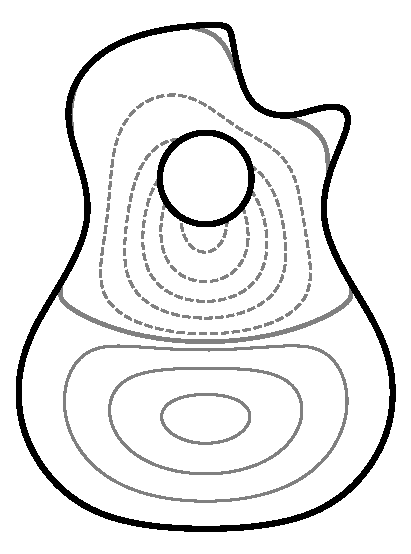
\includegraphics[width=0.2\textwidth]{../pictures/guitar/cutaway-eigfunc1.pdf}%
      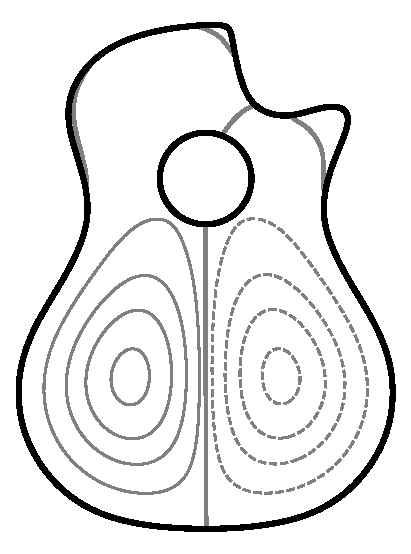
\includegraphics[width=0.2\textwidth]{../pictures/guitar/cutaway-eigfunc2.pdf}%
      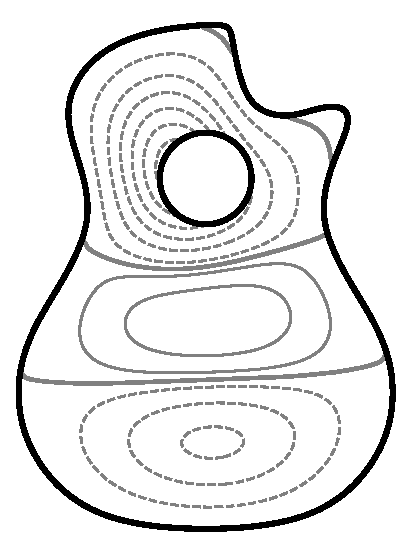
\includegraphics[width=0.2\textwidth]{../pictures/guitar/cutaway-eigfunc3.pdf}%
      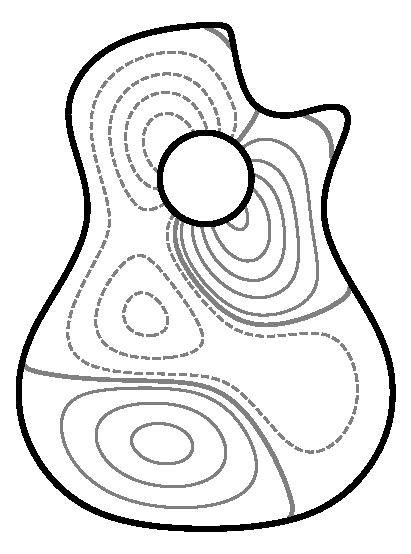
\includegraphics[width=0.2\textwidth]{../pictures/guitar/cutaway-eigfunc4.pdf}%
      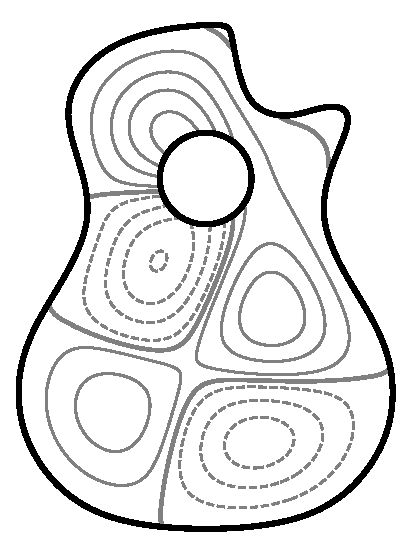
\includegraphics[width=0.2\textwidth]{../pictures/guitar/cutaway-eigfunc5.pdf}
      \\
      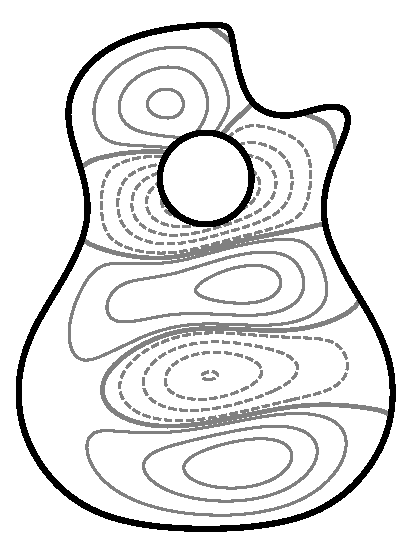
\includegraphics[width=0.2\textwidth]{../pictures/guitar/cutaway-eigfunc8.pdf}%
      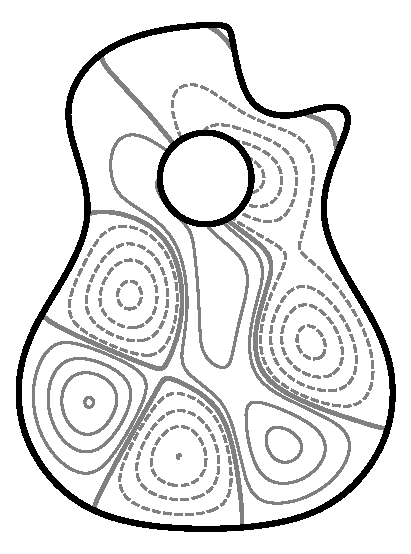
\includegraphics[width=0.2\textwidth]{../pictures/guitar/cutaway-eigfunc9.pdf}%
      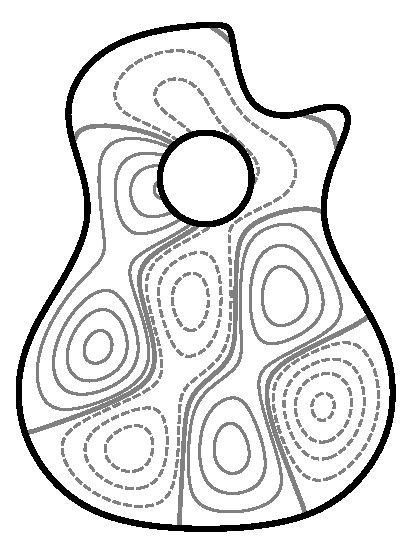
\includegraphics[width=0.2\textwidth]{../pictures/guitar/cutaway-eigfunc10.pdf}%
      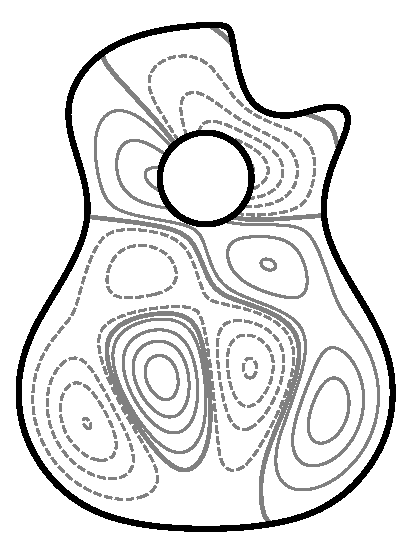
\includegraphics[width=0.2\textwidth]{../pictures/guitar/cutaway-eigfunc11.pdf}%
      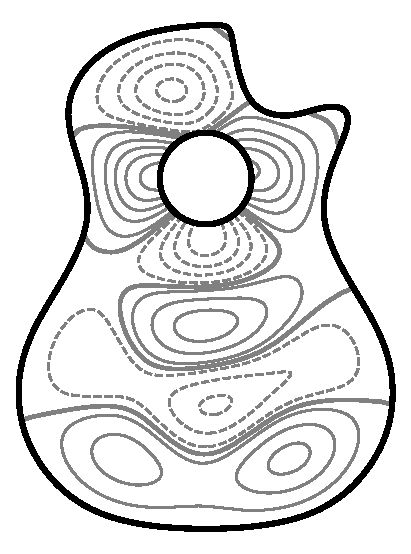
\includegraphics[width=0.2\textwidth]{../pictures/guitar/cutaway-eigfunc12.pdf}
      \\
      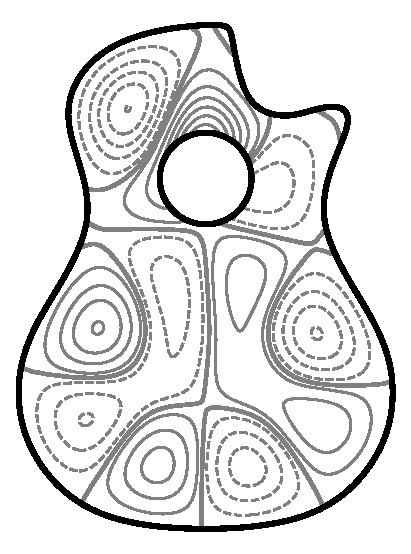
\includegraphics[width=0.2\textwidth]{../pictures/guitar/cutaway-eigfunc15.pdf}%
      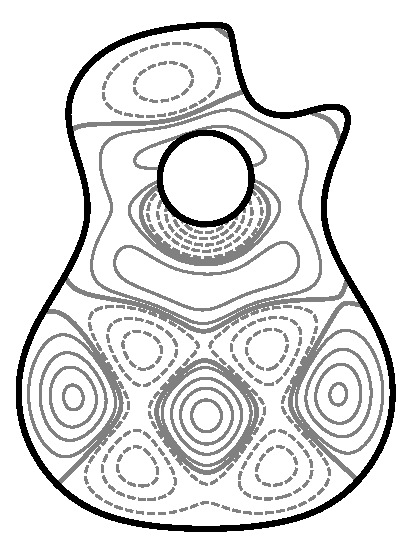
\includegraphics[width=0.2\textwidth]{../pictures/guitar/cutaway-eigfunc16.pdf}%
      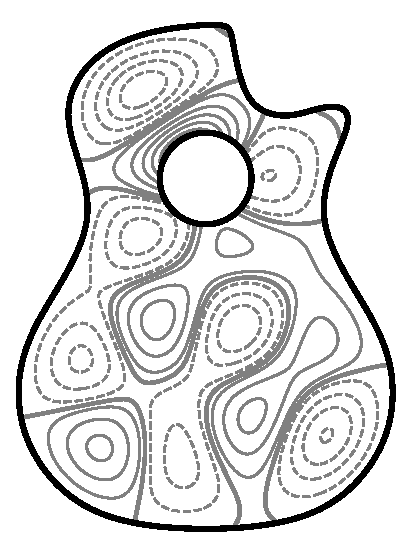
\includegraphics[width=0.2\textwidth]{../pictures/guitar/cutaway-eigfunc17.pdf}%
      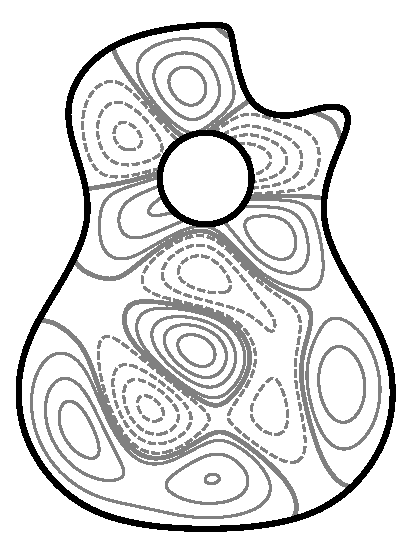
\includegraphics[width=0.2\textwidth]{../pictures/guitar/cutaway-eigfunc18.pdf}%
      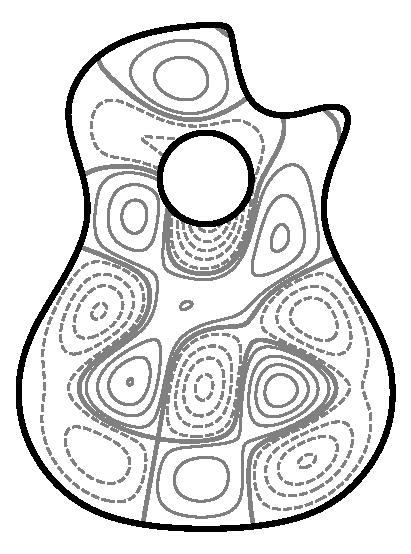
\includegraphics[width=0.2\textwidth]{../pictures/guitar/cutaway-eigfunc19.pdf}
      \\[1em]
      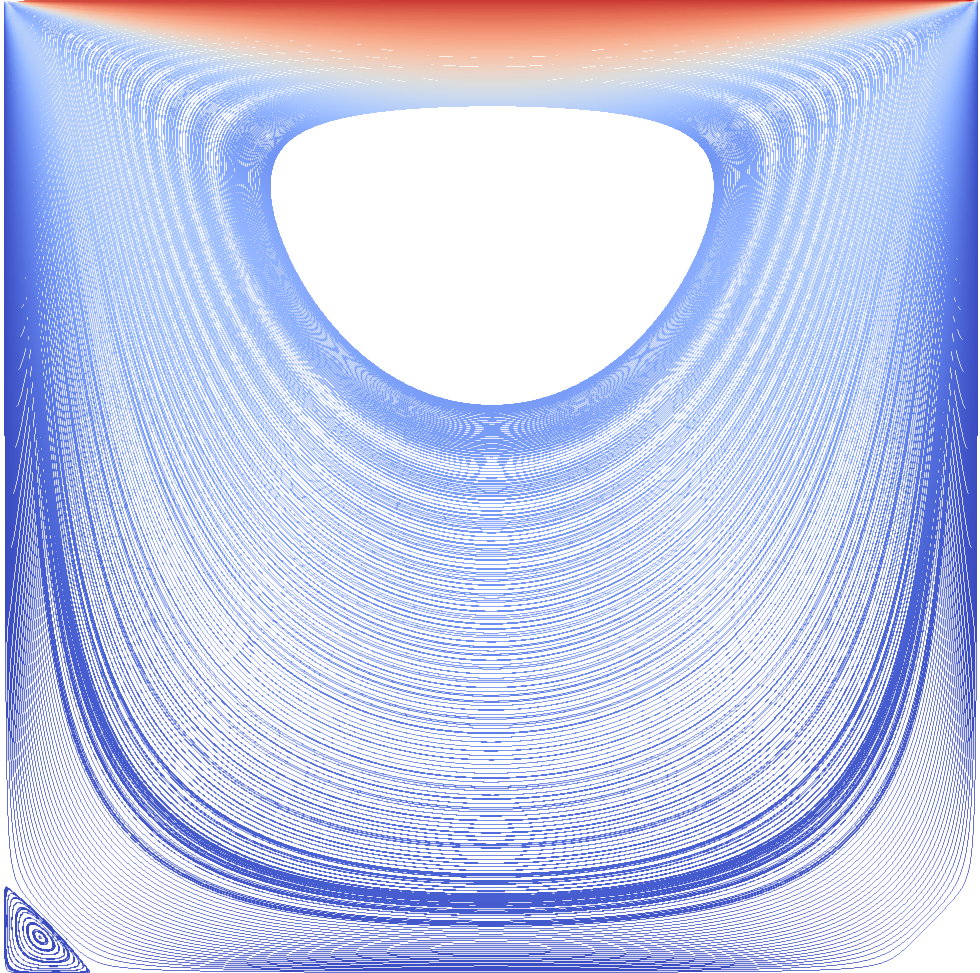
\includegraphics[width=0.333\textwidth]{../pictures/mhd/ldc_1_1_u}%
      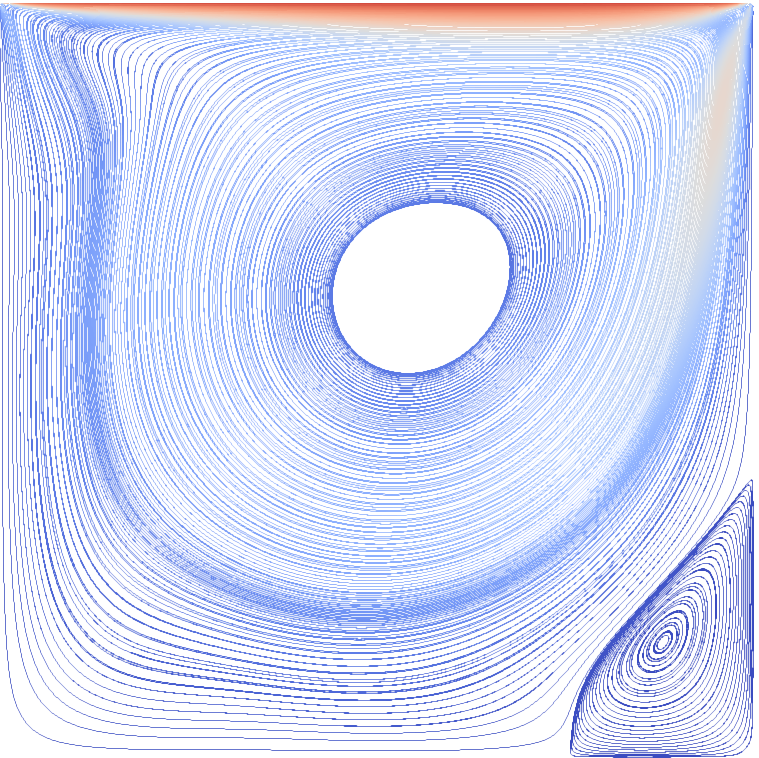
\includegraphics[width=0.333\textwidth]{../pictures/mhd/ldc_500_500_u}%
      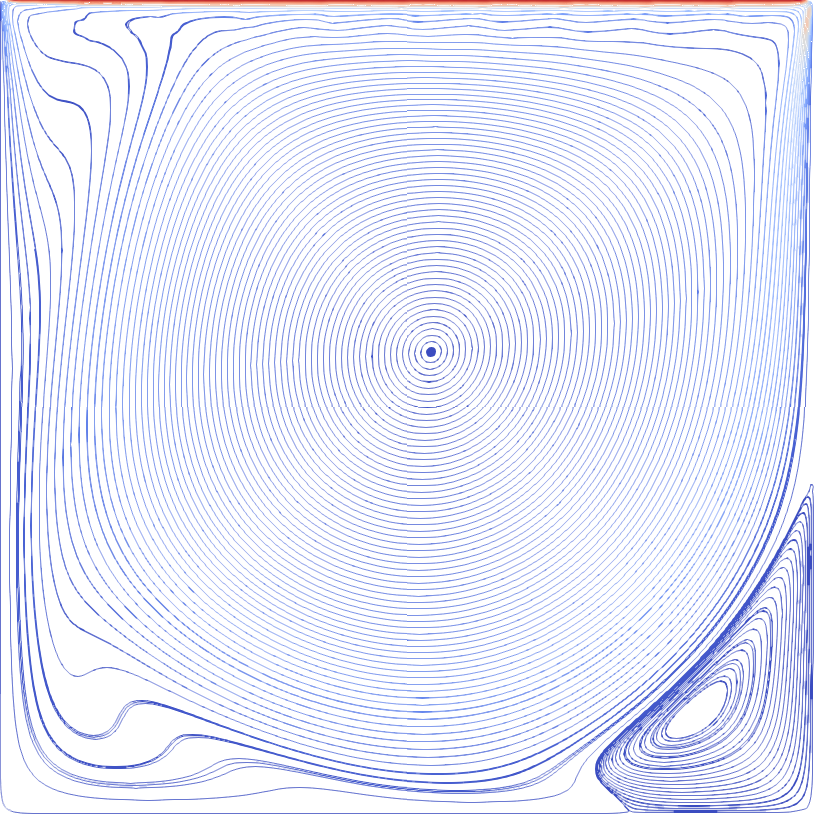
\includegraphics[width=0.333\textwidth]{../pictures/mhd/ldc_5000_5000_u}%
      \\
      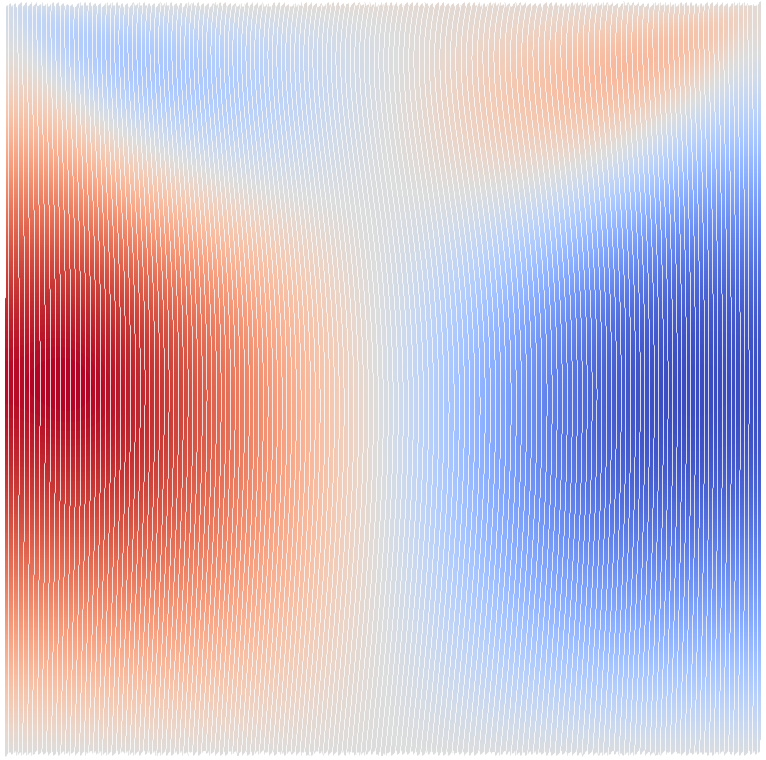
\includegraphics[width=0.333\textwidth]{../pictures/mhd/ldc_1_1_B}%
      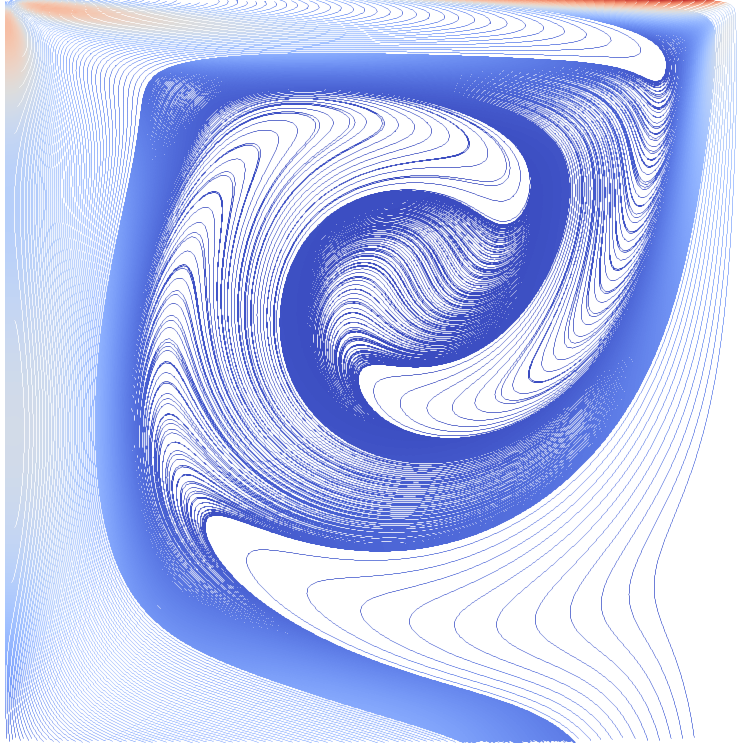
\includegraphics[width=0.333\textwidth]{../pictures/mhd/ldc_500_500_B}%
      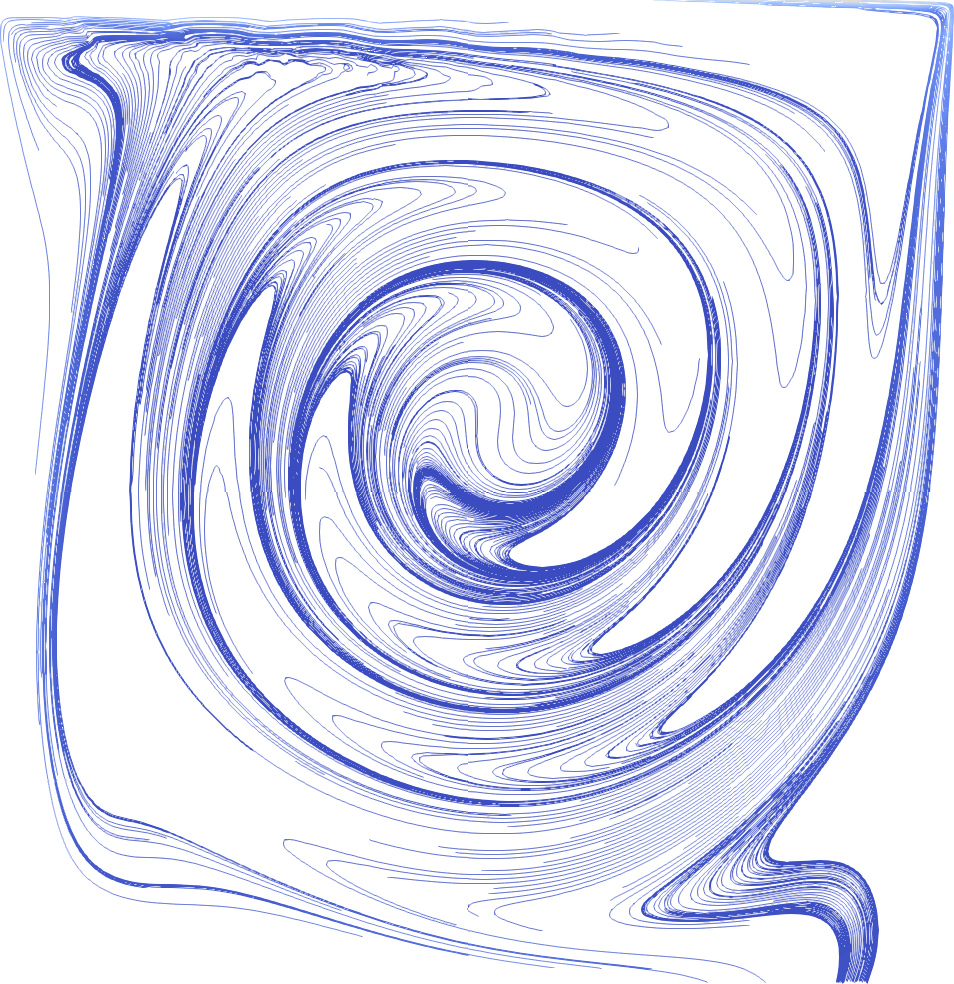
\includegraphics[width=0.333\textwidth]{../pictures/mhd/ldc_5000_5000_B}%
    \end{column}
  \end{columns}
\end{frame}

\section{Automated finite elements}

\begin{frame}
  \frametitle{Firedrake \url{www.firedrakeproject.org}}
  \begin{columns}
    \begin{column}{0.8\textwidth}
      \begin{quote}
        {\normalfont [\ldots]} an automated system for the solution of
        partial differential equations using the finite element
        method.
      \end{quote}
    \end{column}
    \begin{column}{0.2\textwidth}
      
\includegraphics[width=0.8\textwidth]{firedrake}
    \end{column}
  \end{columns}
  \begin{overlayarea}{\textwidth}{0.6\textheight}
    \begin{onlyenv}<1>
      \begin{itemize}
      \item Written in Python.
      \item Finite element problems specified with \emph{embedded}
        domain specific language, UFL from the FEniCS project.
      \item Domain-specific optimising compiler.
      \item Flexible preconditioning framework for problem-specific multigrid and block preconditioners.
      \end{itemize}
      \begin{flushright}
        {\scriptsize F.~Rathgeber, D.A.~Ham, \textbf{L.~Mitchell}, M.~Lange,
        F.~Luporini, A.T.T.~McRae, G.-T.~Bercea, G.R.~Markall,
        P.H.J.~Kelly. ACM Transactions on Mathematical Software
        (2016). \arxivlink{1501.01809}{cs.MS}\nocite{Rathgeber:2016}

      R.C.~Kirby and \textbf{L.~Mitchell}, SIAM SISC (2018). \arxivlink{1706.01346}{cs.MS}\nocite{Kirby:2018}}
    \end{flushright}
  \end{onlyenv}
  \begin{onlyenv}<2>
    \begin{itemize}
    \item ExCALIBUR exascale working group code (continuum mechanics)
    \item Numerics/data structures prototypes for UK Met Office next
      gen dynamical core (Gung-Ho)
    \end{itemize}
    \begin{block}{User groups at}
      Imperial, Oxford, Bath, Leeds, Durham, Kiel, Rice, Houston,
      Exeter, Buffalo, Waterloo, Washington, Baylor, Edinburgh, ANU, \dots

      Contributors from 15 institutions in the last year.
    \end{block}
  \end{onlyenv}
\end{overlayarea}
\end{frame}

\begin{frame}[fragile]
  \frametitle{Code that captures mathematical structure}
  \begin{columns}
    \begin{column}{0.5\framewidth}
      Stationary Rayleigh--B\'enard convection, find $(u, p, T) \in V\times W\times Q$ s.t.
        \begin{align*}
          {\big(\nabla u, \nabla v\big)}_{L_2} + {\big((u \cdot \nabla u), v\big)}_{L_2} \\
          - {\big(p, \nabla\cdot v\big)}_{L_2} + \frac{\text{Ra}}{\text{Pr}}
          {\big(Tg\hat{z}, v\big)}_{L_2} &= 0 \\
          {\big(\nabla\cdot u, q\big)}_{L_2} &= 0\\
          {\big(u \cdot \nabla T, S\big)}_{L_2}
          + \text{Pr}^{-1} {\big(\nabla T, \nabla S\big)}_{L_2} &= 0\\
          \quad \forall\, (v,q,T) \in V\times W \times Q
        \end{align*}
    \end{column}
      \begin{column}{0.5\framewidth}
\begin{minted}[fontsize=\scriptsize]{python}
from firedrake import *
mesh = Mesh(...)
V = VectorFunctionSpace(mesh, "CG", 2)
W = FunctionSpace(mesh, "CG", 1)
Q = FunctionSpace(mesh, "CG", 1)
Z = V * W * Q
Ra = Constant(...)
Pr = Constant(...)
upT = Function(Z)
u, p, T = split(upT)
v, q, S = TestFunctions(Z)
bcs = [...]

F = (inner(grad(u), grad(v))
     + inner(dot(grad(u), u), v)
     - inner(p, div(v))
     + (Ra/Pr)*inner(T*g*zhat, v)
     + inner(div(u), q)
     + inner(dot(grad(T), u), S)
     + (1/Pr)*inner(grad(T), grad(S)))*dx

solve(F == 0, upT, bcs=bcs)
\end{minted}
      \end{column}
  \end{columns}
\end{frame}

\begin{frame}
  \frametitle{Code generation for high performance}
  \begin{columns}
    \begin{column}{0.4\textwidth}
      \begin{itemize}
      \item High-level interface + domain-specific compiler
        optimisations
      \item Optimal complexity finite element assembly
      \item Code generation delivers high performance implementation ($>50\%$ peak)
      \end{itemize}
    \end{column}
    \begin{column}{0.6\textwidth}
      \begin{flushright}
        \begin{tikzpicture}
          \begin{loglogaxis}[
            height=0.4\textheight,
            width=\textwidth,
            name=plot,
            xlabel=Polynomial degree,
            title={Residual assembly on hexes},
            title style={font=\tiny, yshift=-10pt},
            ylabel=FLOPs, xtick={1,2,4,8,16,32},
            xticklabels={$1$,$2$,$4$,$8$,$16$,$32$}, axis lines=left, axis
            line style={-}, log basis x=2,
            xticklabel style={font=\tiny},
            yticklabel style={font=\tiny},
            ylabel style={font=\tiny, yshift=-5pt},
            xlabel style={font=\tiny, yshift=5pt},
            legend cell align=left,
            legend pos=north west,
            legend style={font=\tiny,draw=none, fill=none}]
            \pgfplotstableread[row sep=crcr]{
              degree flops_vanilla flops_opt\\
              1 9.78100e+03 6.48100e+03\\
              2 1.05624e+05 2.78280e+04\\
              3 6.04110e+05 7.50860e+04\\
              4 2.36102e+06 1.63395e+05\\
              5 7.20724e+06 3.09060e+05\\
              6 1.85105e+07 5.33483e+05\\
              7 4.18644e+07 8.60322e+05\\
              8 8.59101e+07 1.31626e+06\\
              9 1.63287e+08 1.93100e+06\\
              10 2.91712e+08 2.73728e+06\\
              11 4.95190e+08 3.77084e+06\\
              12 8.05352e+08 5.07047e+06\\
              13 1.26293e+09 6.67796e+06\\
              14 1.91933e+09 8.63816e+06\\
              15 2.83841e+09 1.09989e+07\\
              16 4.09829e+09 1.38110e+07\\
              17 5.79335e+09 1.71285e+07\\
              18 8.03637e+09 2.10082e+07\\
              19 1.09608e+10 2.55101e+07\\
              20 1.47229e+10 3.06972e+07\\
              21 1.95048e+10 3.66353e+07\\
              22 2.55164e+10 4.33937e+07\\
              23 3.29987e+10 5.10443e+07\\
              24 4.22266e+10 5.96621e+07\\
              25 5.35115e+10 6.93253e+07\\
              26 6.72053e+10 8.01150e+07\\
              27 8.37026e+10 9.21153e+07\\
              28 1.03445e+11 1.05413e+08\\
              29 1.26924e+11 1.20099e+08\\
              30 1.54686e+11 1.36267e+08\\
              31 1.87334e+11 1.54011e+08\\
              32 2.25533e+11 1.73433e+08\\
            }\data; \pgfplotstableset{create on use/vanilla/.style={create
                col/expr={1e3*pow(\thisrow{degree},6)}}};
            \pgfplotstableset{create on use/spectral/.style={create
                col/expr={5e2*pow(\thisrow{degree},4)}}};

            \addplot+[mark=none, color=black, dashed, line width=1.5pt] table
            [x=degree,y=flops_opt] \data;
            \addlegendentry{Sum factorised};
            
            \addplot+[mark=none, color=black, line width=1.5pt] table
            [x=degree,y=flops_vanilla] \data;
            \addlegendentry{Na\"ive};

            \addplot+[mark=none, color=black,
            dotted, line width=1pt] table [x=degree,y=vanilla] \data
            coordinate [pos=0.67] (A);
            \node at (A) [anchor=south east]
            {\footnotesize $\mathcal{O}(p^6)$};

            \addplot+[mark=none, color=black,
            dotted, line width=1pt] table [x=degree,y=spectral] \data
            coordinate [pos=0.67] (B);

            \node at (B) [anchor=north west]
            {\footnotesize $\mathcal{O}(p^4)$};
          \end{loglogaxis}
        \end{tikzpicture}

        
        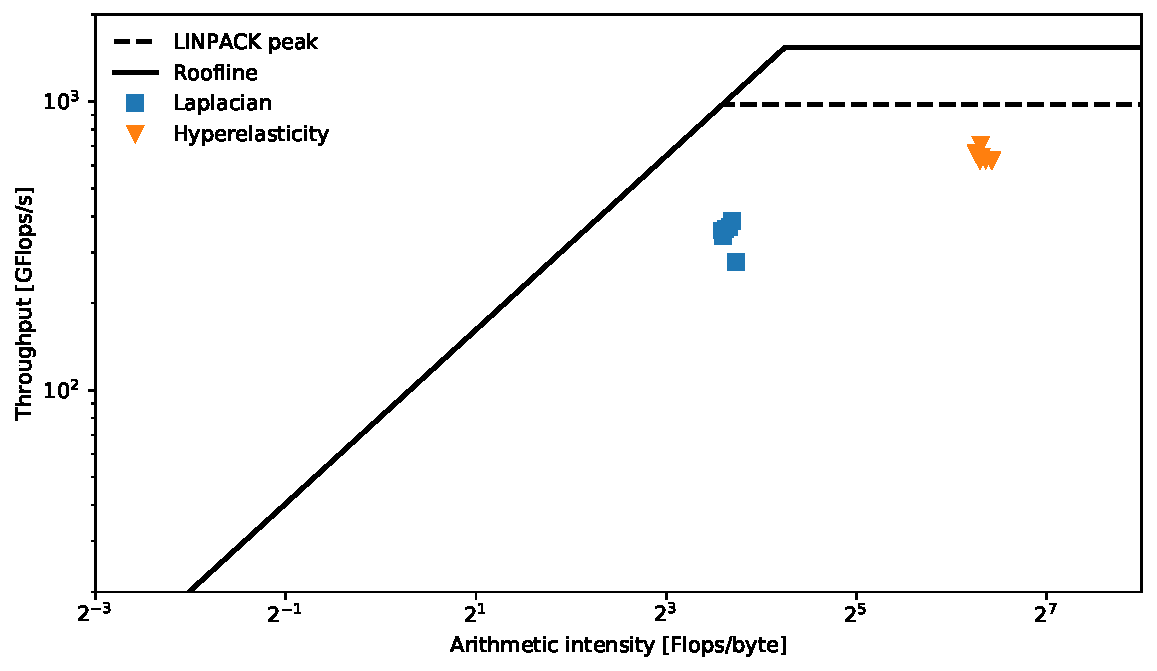
\includegraphics[height=0.4\textheight]{vector-roofline}
        \end{flushright}
    \end{column}
  \end{columns}
  \begin{flushright}
    {\scriptsize M.~Homolya, \textbf{L.~Mitchell}, F.~Luporini,
      D.A.~Ham, SIAM SISC (2018), \arxivlink{1705.03667}{cs.MS}

    T.~Sun, \textbf{L.~Mitchell}, K.~Kulkarni,
    A.~Kl\"ockner, D.A.~Ham, P.H.J.~Kelly, Int. J. HPCA (2020).
      \arxivlink{1903.08243}{cs.MS}}
  \end{flushright}
\end{frame}

\begin{frame}
  \frametitle{Application: coastal ocean modelling}
  \begin{columns}
    \begin{column}{0.55\textwidth}
      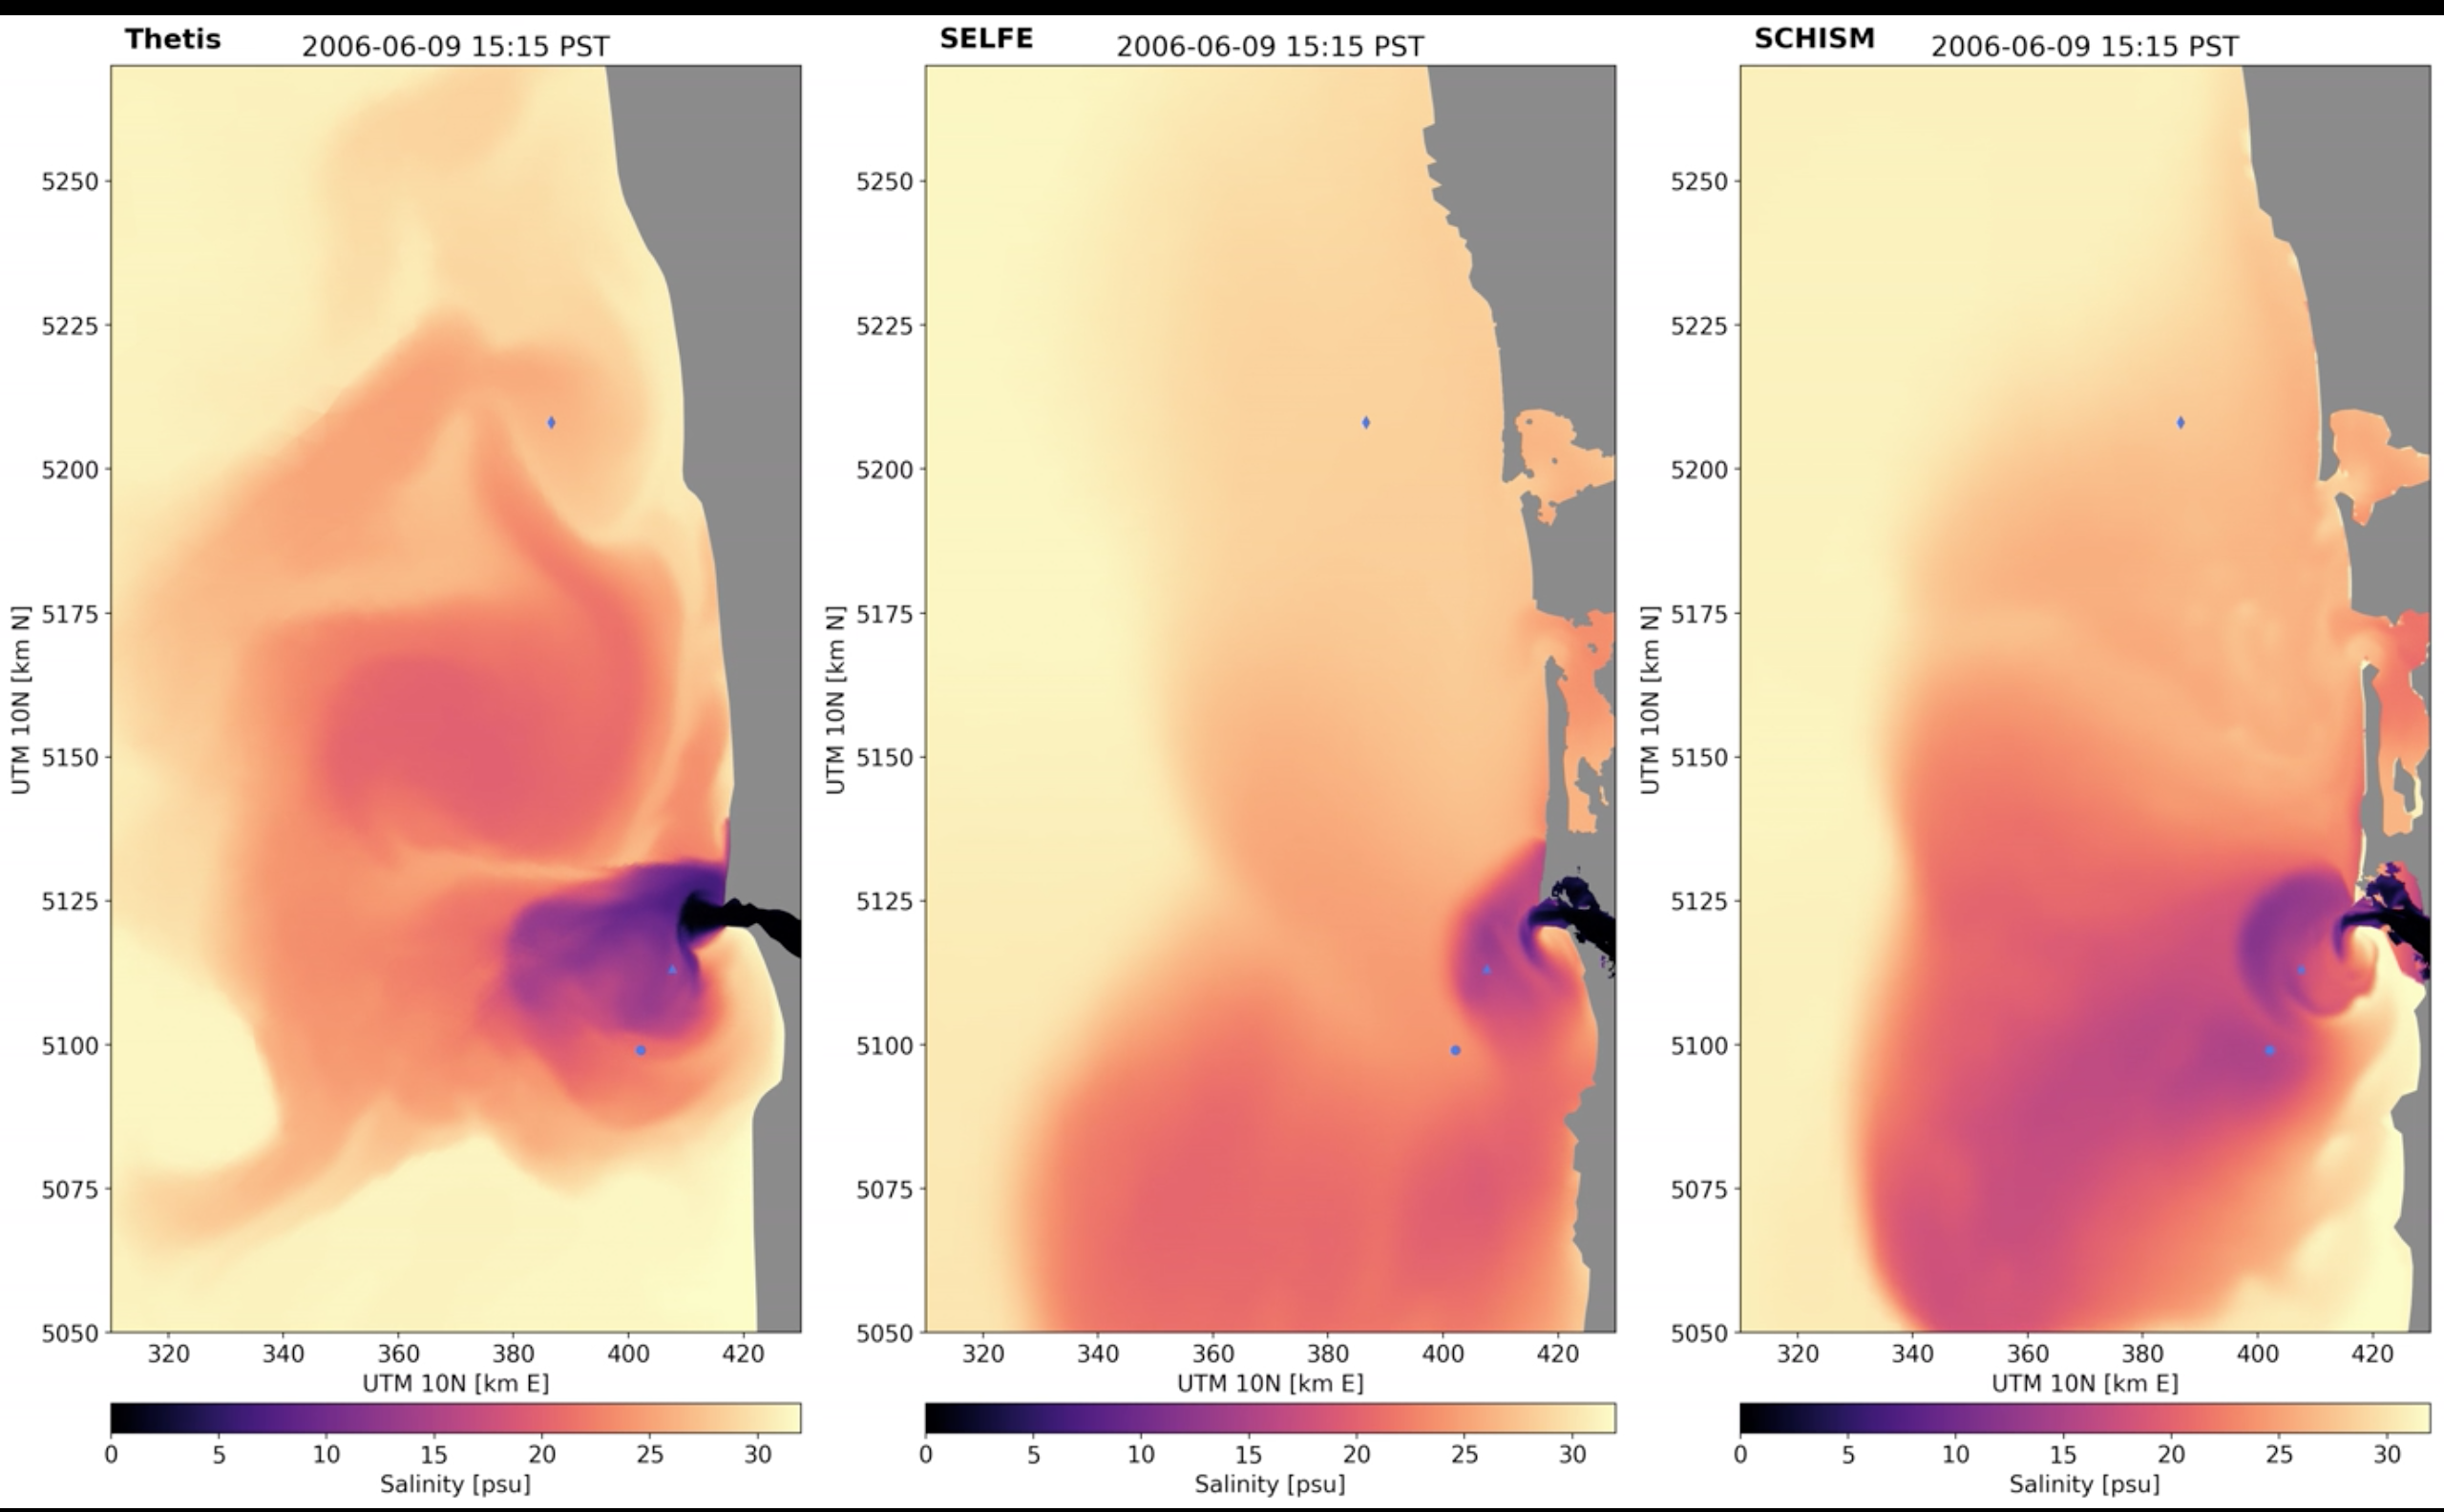
\includegraphics[height=0.45\textheight]{thetis-snapshot}

      {\tiny Surface salinity of the Columbia river plume. Credit
        T.~K\"arn\"a, Finnish Meteorological Institute}
    \end{column}
    \hspace{-0.04\textwidth}
    \begin{column}{0.48\textwidth}
      \begin{itemize}
      \item Lower numerical mixing, improved results.
      \item 3-8x faster than models with similar quality of results.
      \item Differentiable: efficient adjoint.
      \item Used at Finnish Met Institute; Earth Sciences at
        Imperial.
      \item \url{thetisproject.org}
       \end{itemize}
    \end{column}
  \end{columns}
  \begin{flushright}
    {\scriptsize T.~K\"arn\"a, S.C.~Kramer, \textbf{L.~Mitchell}, D.A.~Ham,
      M.D.~Piggott, A.M.~Baptista. Geoscientific Model Development
      (2018).
      \arxivlink{1711.08552}{physics.ao-ph}\nocite{Karna:2018}}
  \end{flushright}
\end{frame}


\section{Augmented Lagrangian preconditioning}

\begin{frame}
  \frametitle{Application challenge}
  \begin{block}{Stationary incompressible Navier--Stokes}
    For $\nu \in \mathbb{R}_+$, find $(u, p) \in \honev \times \ltwo$ such that
    \begin{alignat*}{2}
      - \div (2\nu\eps{u}) + \advect{u}{u} + \nabla p &= f \quad && \text{ in } \Omega, \label{eqn:momentum} \\
      \div u &= 0 \quad && \text{ in } \Omega, \\
      u &= g \quad && \text{ on } \Gamma_D, \\
      2 \nu \eps{u} \cdot n &= pn \quad && \text{ on } \Gamma_N,
    \end{alignat*}
  \end{block}
  \begin{answer}{Headline result}
    Preconditioner with \emph{viscosity-robust} performance in 2D \& 3D.
  \end{answer}

  Uses augmented Lagrangian to control Schur complement, non-nested
  multigrid, $\operatorname{ker}\div$-capturing multigrid relaxation, \dots
\end{frame}

\begin{frame}[fragile]
  \frametitle{Discretisation}
  Scott--Vogelius $(\mathbb{CG}_k)^{d}-\mathbb{DG}_{k-1}$ elements on
  barycentric grids

  \begin{center}
    \includestandalone[width=0.5\textwidth]{../pictures/bary-hierarchy}
  \end{center}

  This is a \emph{structure-preserving} element pair, discretising the
  Stokes complex.

  \begin{center}
    \begin{tikzcd}
      H^2 \arrow[r, "\curl"] \arrow[d] & \mathbf{H}^1 \arrow[r,
      "\div"]
      \arrow[d] & L^2 \arrow[d] \\
      \mathbb{HCT}_{k+1} \arrow[r, "\curl"] & (\mathbb{CG}_k)^2
      \arrow[r, "\div"] & \mathbb{DG}_{k-1}
    \end{tikzcd}
  \end{center}
\end{frame}

\begin{frame}
  \frametitle{Idea: augmented Lagrangian to control Schur complement}
  \begin{exampleblock}{Augmented momentum equation}
    Add $-\gamma \grad\div u$ term to the momentum equation.

    \begin{equation*}
      - \div (2\nu\eps{u}) + \advect{u}{u} + \nabla p -\gamma \grad \div u = f
    \end{equation*}

    Controls Schur complement without changing solution.
  \end{exampleblock}
  \pause
  \begin{challenge}{Problem}
    Normal multigrid applied to linearised augmented momentum operator
    doesn't work, gets worse as $\gamma \to \infty$.

    $\grad\div u$ has an enormous kernel $\Rightarrow$ need a
    specialised multigrid scheme.
  \end{challenge}
\end{frame}


\begin{frame}
  \frametitle{$\gamma$-robust multigrid relaxation}
  Consider the problem: for
  $\alpha, \beta \in \mathbb{R}$, find $u \in V$ such that
  \begin{equation*}
    \alpha a(u, v) + \beta b(u, v) = (f, v) \quad \forall v \in V,
  \end{equation*}
  where $a$ is SPD, and $b$ is symmetric positive semidefinite.

  This matches our problem (ignoring advection) with $a = (\eps{u},
  \eps{v})$ and $b = (\div u, \div v)$.
  \pause
  \begin{theorem}[Sch\"oberl (1999); Lee, Wu, Xu, Zikatanov (2007)]
    {\small
    Let the kernel be
    \begin{equation*}
      \mathcal{N} := \{ u \in V : b(u, v) = 0 \,\, \forall v \in V \}.
    \end{equation*}
    A Schwarz smoother whose decomposition $V = \sum_i
    V_i$ satisfies
    \begin{equation*}
      \mathcal{N} = \sum_i \mathcal{N} \cap V_i,
    \end{equation*}
    is robust wrt $\alpha$ and $\beta$.
    \nocite{Schoeberl:1999,Lee:2007}
    }
  \end{theorem}
\end{frame}

\begin{frame}[fragile]
  \frametitle{Picking the decomposition}
  In 2D, the Stokes complex and S--V subcomplex are
  \begin{center}
    \begin{tikzcd}
      H^2 \arrow[r, "\curl"] \arrow[d] & \mathbf{H}^1 \arrow[r,
      "\div"]
      \arrow[d] & L^2 \arrow[d] \\
      \mathbb{HCT}_{k+1} \arrow[r, "\curl"] & (\mathbb{CG}_k)^2
      \arrow[r, "\div"] & \mathbb{DG}_{k-1}
    \end{tikzcd}
    \includestandalone[width=0.52\textwidth]{../pictures/HCT-complex}
  \end{center}
  giving a \emph{macrostar} decomposition around each vertex in the mesh.
  \begin{center}
    \includestandalone[height=0.3\textheight]{../pictures/macro-star}
  \end{center}
\end{frame}

\begin{frame}
  \frametitle{Structure of full solver}
  \resizebox{\textwidth}{!}{%
    \begin{tikzpicture}[%
  every node/.style={draw=black, thick, anchor=west},
  grow via three points={one child at (0.0,-0.7) and
  two children at (0.0,-0.7) and (0.0,-1.4)},
  edge from parent path={(\tikzparentnode.210) |- (\tikzchildnode.west)}]
  \node {Continuation}
    child { node {Newton solver with line search}
      child { node {Krylov solver (FGMRES)}
        child { node {Block preconditioner}
          child { node {Approximate Schur complement inverse}
              child { node {Exact pressure mass matrix inverse}}
          }
          child [missing] {}
          child { node {F-cycle on augmented momentum block}
              child { node {Coarse grid solver}
                child { node {LU factorization}}
              }
              child [missing] {}
              child { node {Prolongation operator}
                child { node {Local solves over coarse macro cells}}
              }
              child [missing] {}
              child { node {Relaxation}
                child { node {GMRES}
                  child { node {Additive macrostar iteration}}
                }
              }
          }
        }
      }
    };
\end{tikzpicture}
}
\end{frame}
\begin{frame}
  \frametitle{Numerical results --- 2D lid-driven cavity}
  \begin{table}[htbp]
    \centering
    \begin{tabular}{cc|ccccc}
      \toprule
      \# ref. & \# dofs & \multicolumn{5}{c}{Reynolds number} \\
              && 10 & 100 & 1000 & 5000 & 10000 \\
      \midrule
      1 & $9.3 \times 10^4$ & 2.50 & 2.33 & 2.33 & 5.50 & 8.50 \\
      2 & $3.7 \times 10^5$ & 2.00 & 2.00 & 2.00 & 4.00 & 6.00 \\
      3 & $1.5 \times 10^6$ & 2.00 & 1.67 & 1.67 & 2.50 & 3.50 \\
      4 & $5.9 \times 10^6$ & 2.00 & 1.67 & 1.50 & 1.50 & 4.00 \\
      \bottomrule
    \end{tabular}
    \caption{Average number of outer Krylov iterations per Newton step
      for a 2D regularised lid-driven cavity problem with
      $(\mathbb{CG}_3)^{2}-\mathbb{DG}_2$ pair.}
  \end{table}
  \begin{flushright}
    {\scriptsize
    P.E.~Farrell, \textbf{L.~Mitchell}, L.R.~Scott, and F.~Wechsung,
    SMAI JCM (2021).
    \arxivlink{2004.09398}{math.NA}\nocite{Farrell:2021a}
    }
  \end{flushright}
\end{frame}

\begin{frame}
  \frametitle{Numerical results --- 3D lid-driven cavity}
  \begin{table}[htbp]
    \centering
    \begin{tabular}{cc|ccccc}
      \toprule
      \# ref. & \# dofs & \multicolumn{5}{c}{Reynolds number} \\
              && 10 & 100 & 1\,000 & 2\,500 & 5\,000 \\
      \midrule
      1   & $1.03\times 10^6$     & 3.00  & 3.67  & 3.50 & 4.00 & 5.00\\
      2   & $8.22\times 10^6$     & 3.50  & 3.67  & 4.00 & 4.00 & 4.00\\
      3   & $6.55\times 10^7$     & 3.00  & 3.33  & 3.50 & 3.50 & 4.00\\
      \bottomrule
    \end{tabular}
    \caption{Average number of outer Krylov iterations per Newton step for a
      3D regularised lid-driven cavity problem with
      $(\mathbb{CG}_3)^{2}-\mathbb{DG}_2$ pair.}
  \end{table}
  \begin{flushright}
    {\scriptsize
    P.E.~Farrell, \textbf{L.~Mitchell}, L.R.~Scott, and F.~Wechsung,
    SMAI JCM (2021).
    \arxivlink{2004.09398}{math.NA}\nocite{Farrell:2021a}
    }
  \end{flushright}
\end{frame}

\section{Future directions}


\begin{frame}
  \frametitle{Efficient high-order FEM}

  \begin{challenge}{Challenge}
    High-order methods are excellent fit to modern HPC hardware, and simulation
    challenges.

    Efficient implementation and solution is the domain of a few experts.
  \end{challenge}

  \begin{answer}{Research questions}
    How to deliver usable simulation tools that exploit structure in
    high-order methods?
    \begin{itemize}
    \item For efficient assembly in engineering-relevant applications;
    \item For fast solvers: robust $p$-multigrid.
    \end{itemize}

    $\Rightarrow$ EPSRC Excalibur proposal in review (with Patrick
    Farrell, Dave Moxey, Spencer Sherwin, UKAEA).
  \end{answer}
\end{frame}

\begin{frame}
  \frametitle{Structure-preservation and preconditioning}

  \begin{challenge}{Challenge}
    Parameter-robust preconditioners for coupled problems.

    Toolkit: augmented Lagrangian + subspace correction + Hilbert complexes.
  \end{challenge}
  
  \begin{answer}{Research questions}
    Theory only available for symmetric coercive case. What can we say about
    \begin{itemize}
    \item symmetric indefinite problems?
    \item non-symmetric problems with a kernel?
    \item Coupled all-at-once relaxation?
    \item Constraints other than div- or curl-freeness?
    \end{itemize}

    $\Rightarrow$ NERC proposal in preparation: augmented Lagrangian
    applied to timestepping schemes with mass conservation (with Colin
    Cotter, UK Met Office)
  \end{answer}
\end{frame}

\begin{frame}
  \frametitle{Summary}
  \begin{itemize}
  \item Broad interdisciplinary research agenda spanning:
    \begin{itemize}
    \item finite element discretisation and implementation;
    \item linear and non-linear solvers/preconditioners;
    \item high-performance computing \& domain-specific compilers.
    \end{itemize}
  \item Application areas:
    \begin{itemize}
    \item coastal ocean \& freshwater outflow;
    \item renewable energy;
    \item numerical weather prediction.
    \end{itemize}
  \item Links:
    \begin{itemize}
    \item Dolean, Pestana, Ramage (preconditioning);
    \item Barranchea (FE discretisation);
    \item MSP (programming language design).
    \end{itemize}
  \end{itemize}
\end{frame}

\appendix
\begin{frame}[t,allowframebreaks]
  \frametitle{References}
  \printbibliography[heading=none]
\end{frame}

\end{document}
